\documentclass[main.tex]{subfiles}
\pagestyle{main}

\begin{document}

%%%%%%%% Longueurs pour traiter les scanners  %%%%%%%%%%

\chapter{Tableaux et graphiques complémentaires \label{chap:anx_img_complement}}

\section{Ensemble des données}
L'ensemble des données utilisé pour réaliser ces travaux est présenté dans cette section. L'ensemble des scanners des 2 patients, \Nber et \Chen, est présenté ici. On présentera ensuite l'ensemble des histogrammes des niveaux de gris, correspondant à la zone tumorale contourée manuellement \correction{-- par mes soins --} sur les scanners. \correction{Une étude (présentée dans~\cite{Cornelis2016}), menée par F. Cornelis, a été réalisée pour examiner l'impact de l'observateur sur la segmentation. Il a été demandé à 2 groupes d'observateurs de contourer 6 lésions hépatiques et 7 lésions pulmonaires. Le groupe A est constitué de 10 médecins entrainés à la segmentation tandis que le groupe B (dont j'ai eu le plaisir de faire parti) est formé de 10 scientifiques avec une connaissance basique de la segmentation. 
L'étude statistique réalisée sur la variabilité inter-opérateur et inter-groupe de la segmentation à montrer qu'il n'apparaît aucune différence significative selon l'opérateur ou le groupe. De plus, F. Cornelis, radiologue au CHU de Bordeaux, avec qui nous collaborons, a validé le contourage effectué. Ceci rend légitime mon propre contourage.}

\newpage
%%\section{Ensemble des données}
\subsection{Scanners de \Nber}
\Nber est traité avec de l'imatinib du jour 119 au jour 867, jour où la rechute est constatée. Le sunitinib est ensuite administré, et là aussi le traitement est efficace avant une rechute débutant au jour~1116. Sur la figure ci-dessous, on peut visualiser l'ensemble des scanners réalisés sur ce patient.

%%%%%% scan NBER
\begin{figure}[h!]
\centering\hfill
\subfloat[16 sept. 2008 -- Jour 119]{\label{fig:hen_full_spatial_1}
\reshapeimg{1.0}{0px}{0px}%
\tikzzoom{full_scan/scan_henbert/2008_09_16(2).jpg}{3}{1.5}{1.2}%
}
\subfloat[30 juin 2009 -- Jour 406]{\label{fig:hen_full_spatial_2}
\reshapeimg{1.1}{0px}{-9px}%
\tikzzoom{full_scan/scan_henbert/2009_06_30(2).jpg}{3}{1.6}{1.2}%
}
\subfloat[5 juill. 2010  -- Jour 776]{\label{fig:hen_full_spatial_3}
\reshapeimg{1.1}{0px}{28px}%
\tikzzoom{full_scan/scan_henbert/2010_07_05(3).jpg}{3}{1.5}{1.0}%
}
\\
\subfloat[25 oct. 2010 -- Jour 888]{\label{fig:hen_full_spatial_4}
\reshapeimg{1.28}{45px}{50px}%
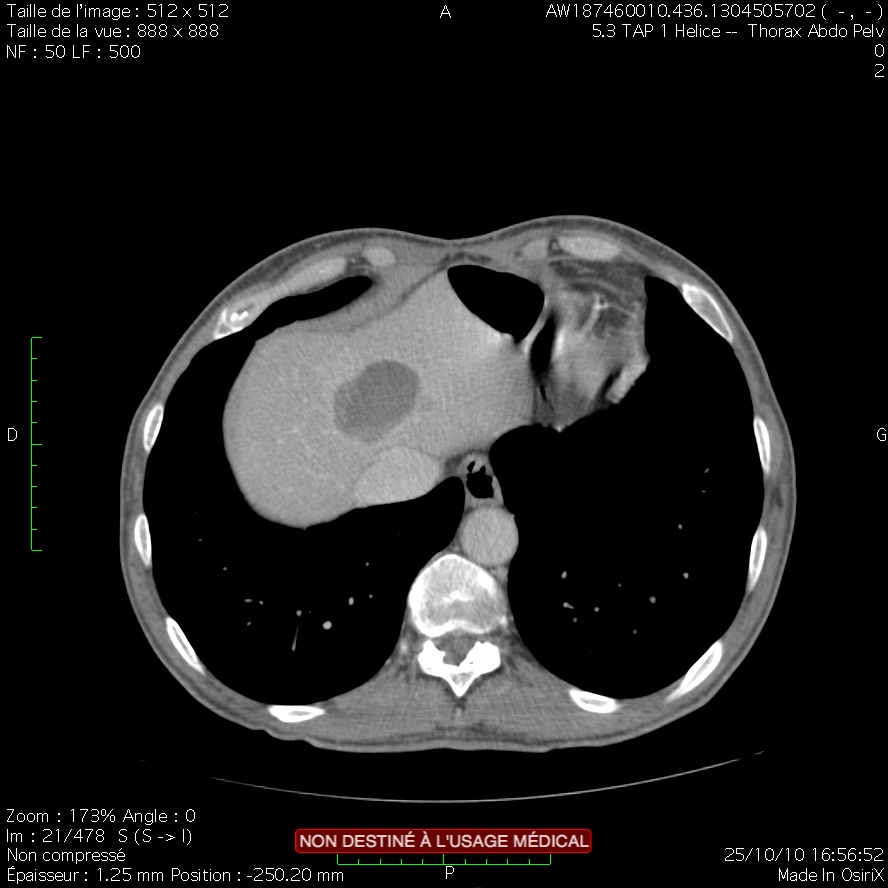
\includegraphics[trim = {\margg} {\margb} {\margd} {\margh}, clip, width=0.32\textwidth]{full_scan/scan_henbert/2010_10_25.jpg}%
}
\subfloat[7 janv. 2011 -- Jour 962]{\label{fig:hen_full_spatial_5}
\reshapeimg{1.11}{20px}{-66px}%
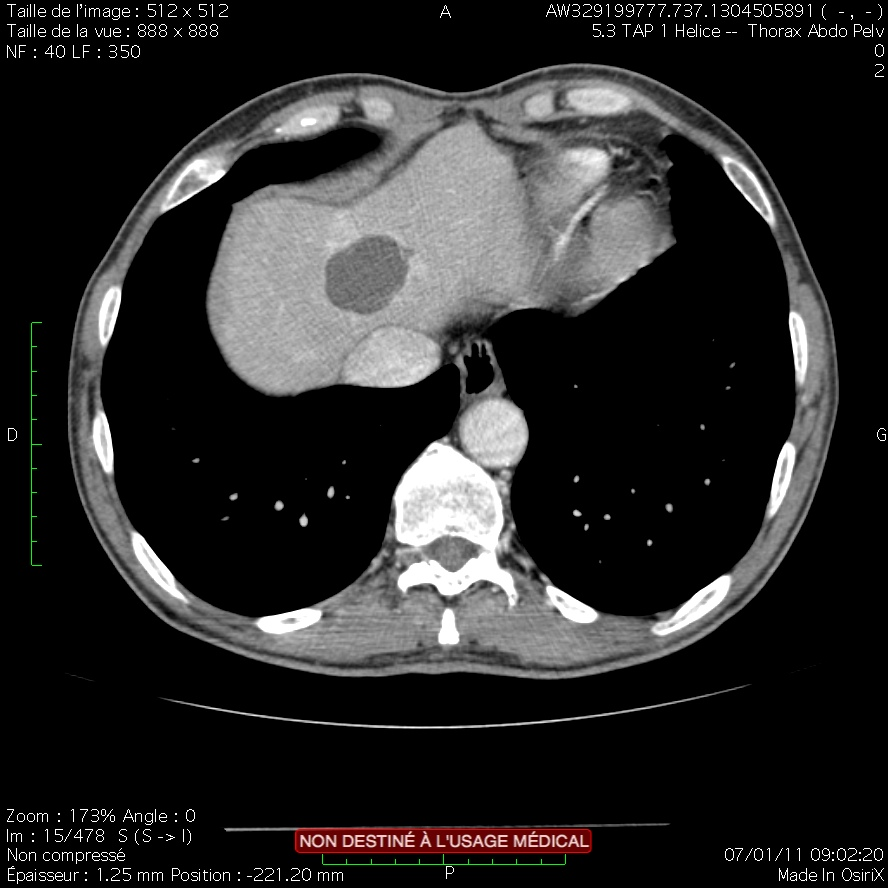
\includegraphics[trim = {\margg} {\margb} {\margd} {\margh}, clip, width=0.32\textwidth]{full_scan/scan_henbert/2011_01_07(2).jpg}%
}
\subfloat[10 juin 2011 -- Jour 1116]{\label{fig:hen_full_spatial_6}
\reshapeimg{1.28}{50px}{-8px}%
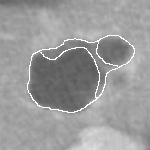
\includegraphics[trim = {\margg} {\margb} {\margd} {\margh}, clip, width=0.32\textwidth]{full_scan/scan_henbert/2011_06_10.jpg}%
}
\caption{\label{fig:nber_complete_scan}Evolution spatiale de la métastase hépatique de \Nber sur une série de scanners.}
\vspace{-5mm}
\end{figure}


\newlength{\largeurfignber}
\setlength{\largeurfignber}{0.19\textwidth}
%\begin{figure}
%\centering
%\subfloat[Jour 0]{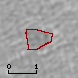
\includegraphics[width=\largeurfignber]{dcm_img/Nber_2008_05_20_scan_contour.png}}\ 
%\subfloat[Jour 119]{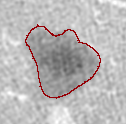
\includegraphics[width=\largeurfignber]{dcm_img/Nber_2008_09_16_scan_contour.png}}\ 
%\subfloat[Jour 209]{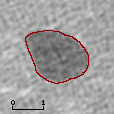
\includegraphics[width=\largeurfignber]{dcm_img/Nber_2008_12_15_scan_contour.png}}\ 
%\subfloat[Jour 275]{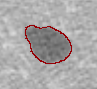
\includegraphics[width=\largeurfignber]{dcm_img/Nber_2009_02_19_scan_contour.png}}\ 
%\subfloat[Jour 331]{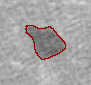
\includegraphics[width=\largeurfignber]{dcm_img/Nber_2009_04_16_scan_contour.png}}\ 
%\subfloat[Jour 406]{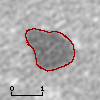
\includegraphics[width=\largeurfignber]{dcm_img/Nber_2009_06_30__slice-244_85_scan_contour.png}}\ 
%\subfloat[Jour 493]{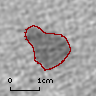
\includegraphics[width=\largeurfignber]{dcm_img/Nber_2009_09_25_scan_contour.png}}\ 
%\subfloat[Jour 535]{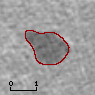
\includegraphics[width=\largeurfignber]{dcm_img/Nber_2009_11_06_scan_contour.png}}\ 
%\subfloat[Jour 611]{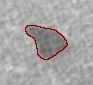
\includegraphics[width=\largeurfignber]{dcm_img/Nber_2010_01_21_scan_contour.png}}\ 
%\subfloat[Jour 688]{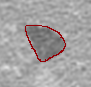
\includegraphics[width=\largeurfignber]{dcm_img/Nber_2010_04_08_scan_contour.png}}\ 
%\subfloat[Jour 776]{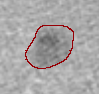
\includegraphics[width=\largeurfignber]{dcm_img/Nber_2010_07_05__slice-263_20_scan_contour.png}}\ 
%\subfloat[Jour 867]{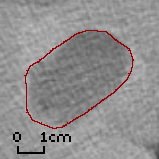
\includegraphics[width=\largeurfignber]{dcm_img/Nber_2010_10_04__slice-239_40_scan_contour.png}}\ 
%\subfloat[Jour 888]{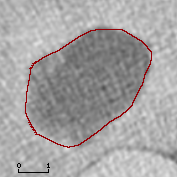
\includegraphics[width=\largeurfignber]{dcm_img/Nber_2010_10_25__slice-246_60_scan_contour.png}}\ 
%\subfloat[Jour 927]{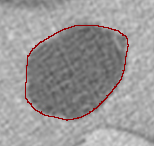
\includegraphics[width=\largeurfignber]{dcm_img/Nber_2010_12_03_scan_contour.png}}\ 
%\subfloat[Jour 962]{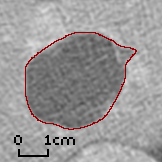
\includegraphics[width=\largeurfignber]{dcm_img/Nber_2011_01_07__slice-221_20_scan_contour.png}}\ 
%\subfloat[Jour 990]{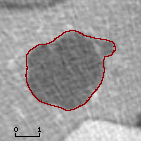
\includegraphics[width=\largeurfignber]{dcm_img/Nber_2011_02_04_scan_contour.png}}\ 
%\subfloat[Jour 1053]{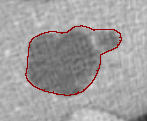
\includegraphics[width=\largeurfignber]{dcm_img/Nber_2011_04_08_scan_contour.png}}\ 
%\subfloat[Jour 1116]{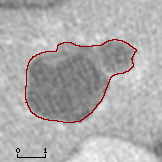
\includegraphics[width=\largeurfignber]{dcm_img/Nber_2011_06_10_scan_contour.png}}\ 
%\subfloat[Jour 1179]{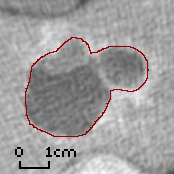
\includegraphics[width=\largeurfignber]{dcm_img/Nber_2011_08_12_scan_contour.png}}
%\caption{\label{fig:contourageNber} Contourage manuel de la tumeur de \Nber. }
%\end{figure}

%\begin{figure}[h!]
\begin{figure}[p]
\captionsetup[subfigure]{labelformat=simple, labelsep=colon}
\renewcommand{\thesubfigure}{\arabic{subfigure}} %% Met des label en numeros (au lieu des lettres)
\addtocounter{subfigure}{-1} %% Commence a 0
\setlength{\tabcolsep}{1mm} %%% padding horizontal
\begin{tabular}{ccccc}
\subfloat[Jour 0]{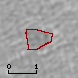
\includegraphics[width=\largeurfignber]{dcm_img/Nber_2008_05_20_scan_contour.png}}&
\subfloat[Jour 119]{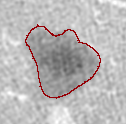
\includegraphics[width=\largeurfignber]{dcm_img/Nber_2008_09_16_scan_contour.png}}&
\subfloat[Jour 209]{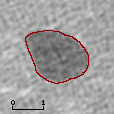
\includegraphics[width=\largeurfignber]{dcm_img/Nber_2008_12_15_scan_contour.png}}&
\multicolumn{2}{c}{%
\multirow{2}{*}[15mm]{
\captionsetup[subfigure]{labelformat=empty}
\vspace{-3cm}
\subfloat[Position des points]{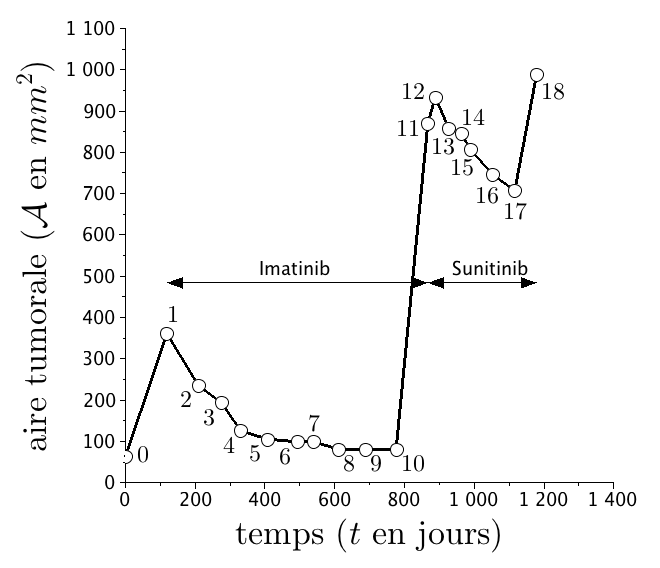
\includegraphics[width=2\largeurfignber]{evo_tps/henbert_listing_point.png}}
\captionsetup[subfigure]{labelformat=parens}
\addtocounter{subfigure}{-1}
}}\\
\subfloat[Jour 275]{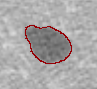
\includegraphics[width=\largeurfignber]{dcm_img/Nber_2009_02_19_scan_contour.png}}&
\subfloat[Jour 331]{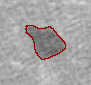
\includegraphics[width=\largeurfignber]{dcm_img/Nber_2009_04_16_scan_contour.png}}&
\subfloat[Jour 406]{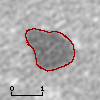
\includegraphics[width=\largeurfignber]{dcm_img/Nber_2009_06_30__slice-244_85_scan_contour.png}}&
\multicolumn{2}{c}{}\\
\subfloat[Jour 493]{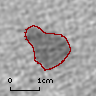
\includegraphics[width=\largeurfignber]{dcm_img/Nber_2009_09_25_scan_contour.png}}&
\subfloat[Jour 535]{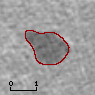
\includegraphics[width=\largeurfignber]{dcm_img/Nber_2009_11_06_scan_contour.png}}&
\subfloat[Jour 611]{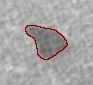
\includegraphics[width=\largeurfignber]{dcm_img/Nber_2010_01_21_scan_contour.png}}&
\subfloat[Jour 688]{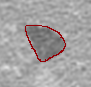
\includegraphics[width=\largeurfignber]{dcm_img/Nber_2010_04_08_scan_contour.png}}&
\subfloat[Jour 776]{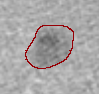
\includegraphics[width=\largeurfignber]{dcm_img/Nber_2010_07_05__slice-263_20_scan_contour.png}}\\
\subfloat[Jour 867]{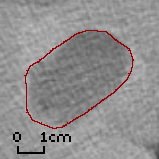
\includegraphics[width=\largeurfignber]{dcm_img/Nber_2010_10_04__slice-239_40_scan_contour.png}}&
\subfloat[Jour 888]{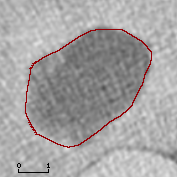
\includegraphics[width=\largeurfignber]{dcm_img/Nber_2010_10_25__slice-246_60_scan_contour.png}}&
\subfloat[Jour 927]{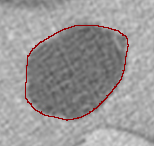
\includegraphics[width=\largeurfignber]{dcm_img/Nber_2010_12_03_scan_contour.png}}&
\subfloat[Jour 962]{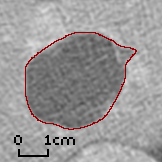
\includegraphics[width=\largeurfignber]{dcm_img/Nber_2011_01_07__slice-221_20_scan_contour.png}}&
\subfloat[Jour 990]{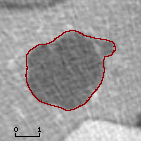
\includegraphics[width=\largeurfignber]{dcm_img/Nber_2011_02_04_scan_contour.png}}\\
&\subfloat[Jour 1053]{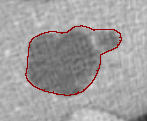
\includegraphics[width=\largeurfignber]{dcm_img/Nber_2011_04_08_scan_contour.png}}&
\subfloat[Jour 1116]{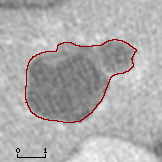
\includegraphics[width=\largeurfignber]{dcm_img/Nber_2011_06_10_scan_contour.png}}&
\subfloat[Jour 1179]{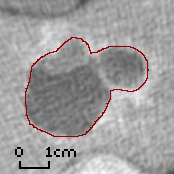
\includegraphics[width=\largeurfignber]{dcm_img/Nber_2011_08_12_scan_contour.png}}
\end{tabular}
\caption{\label{fig:contourageNber} Contourage manuel de la tumeur de \Nber. }
\end{figure}

\FloatBarrier
\newpage
\subsection{Scanners de \Chen}
%\begin{figure}
%\renewcommand{\thesubfigure}{\arabic{subfigure}} %% Met des label en numeros (au lieu des lettres)
%\addtocounter{subfigure}{-1} %% Commence a 0
%\begin{tabular}{ccccc}
%\subfloat[Jour 0]{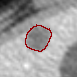
\includegraphics[width=\largeurfignber]{dcm_img/Chen_2007_05_23_scan_contour.png}}&
%\subfloat[Jour 93]{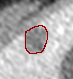
\includegraphics[width=\largeurfignber]{dcm_img/Chen_2007_08_24_scan_contour.png}}&
%\subfloat[Jour 182]{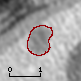
\includegraphics[width=\largeurfignber]{dcm_img/Chen_2007_11_21_scan_contour.png}}\\
%\subfloat[Jour 279]{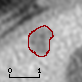
\includegraphics[width=\largeurfignber]{dcm_img/Chen_2008_02_26_scan_contour.png}}&
%\subfloat[Jour 331]{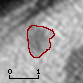
\includegraphics[width=\largeurfignber]{dcm_img/Chen_2008_04_18_scan_contour.png}}&
%\subfloat[Jour 429]{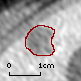
\includegraphics[width=\largeurfignber]{dcm_img/Chen_2008_07_25_scan_contour.png}}&
%\captionsetup[subfigure]{labelformat=empty}
%\subfloat[Position des points]{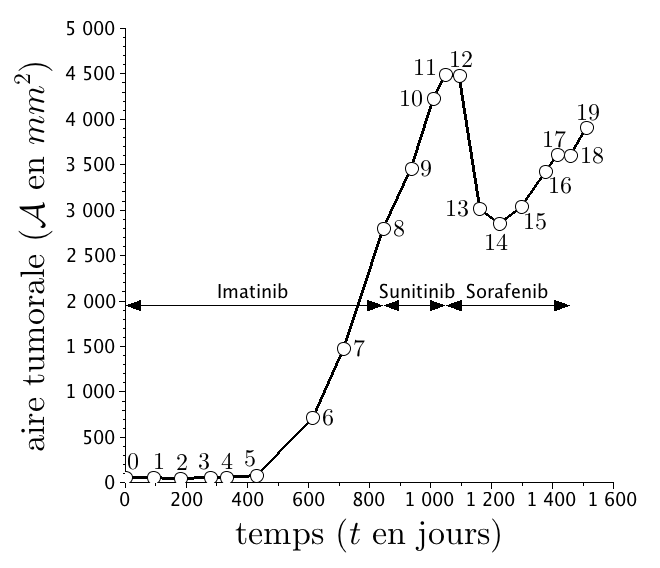
\includegraphics[width=2\largeurfignber]{evo_tps/chen_listing_point.png}}\\
%\captionsetup[subfigure]{labelformat=parens}
%\addtocounter{subfigure}{-1}
%\subfloat[Jour 614]{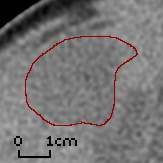
\includegraphics[width=\largeurfignber]{dcm_img/Chen_2009_01_26_scan_contour.png}}&
%\subfloat[Jour 715]{\includegraphics[width=\largeurfignber]{dcm_img/Chen_2009_05_07_scan_contour.png}}&
%\subfloat[Jour 845]{\includegraphics[width=\largeurfignber]{dcm_img/Chen_2009_09_14_scan_contour.png}}&
%\subfloat[Jour 936]{\includegraphics[width=\largeurfignber]{dcm_img/Chen_2009_12_14_scan_contour.png}}&
%\subfloat[Jour 1009]{\includegraphics[width=\largeurfignber]{dcm_img/Chen_2010_02_25_scan_contour.png}}\\
%\subfloat[Jour 1049]{\includegraphics[width=\largeurfignber]{dcm_img/Chen_2010_04_06_scan_contour.png}}&
%\subfloat[Jour 1093]{\includegraphics[width=\largeurfignber]{dcm_img/Chen_2010_05_20_scan_contour.png}}&
%\subfloat[Jour 1161]{\includegraphics[width=\largeurfignber]{dcm_img/Chen_2010_07_27_scan_contour.png}}&
%\subfloat[Jour 1224]{\includegraphics[width=\largeurfignber]{dcm_img/Chen_2010_09_28_scan_contour.png}}&
%\subfloat[Jour 1296]{\includegraphics[width=\largeurfignber]{dcm_img/Chen_2010_12_09_scan_contour.png}}\\
%\subfloat[Jour 1377]{\includegraphics[width=\largeurfignber]{dcm_img/Chen_2011_02_28_scan_contour.png}}& 
%\subfloat[Jour 1415]{\includegraphics[width=\largeurfignber]{dcm_img/Chen_2011_04_07_scan_contour.png}}&
%\subfloat[Jour 1458]{\includegraphics[width=\largeurfignber]{dcm_img/Chen_2011_05_20_scan_contour.png}}& 
%\subfloat[Jour 1510]{\includegraphics[width=\largeurfignber]{dcm_img/Chen_2011_07_11_scan_contour.png}}
%\end{tabular}
%\caption{\label{fig:contourageChen} Contourage manuel de la tumeur de \Chen. }
%\end{figure}

\Chen est d'abord traité à l'imatinib, du jour 0 au jour 845. Après une rechute, le sunitinib est utilisé mais il est totalement inefficace. Au jour~1600, le troisième traitement (sorafénib) est démarré. 
Sur la figure ci-dessous, on peut visualiser l'ensemble des scanners réalisés sur ce patient. \vspace{-1cm}
\begin{figure}[h!]
\captionsetup[subfigure]{labelformat=simple, labelsep=colon}
\renewcommand{\thesubfigure}{\arabic{subfigure}} %% Met des label en numeros (au lieu des lettres)
\addtocounter{subfigure}{-1} %% Commence a 0
\setlength{\tabcolsep}{1mm} %%% padding horizontal
\begin{tabular}{ccccc}
%%% \renewcommand{\arraystretch}{3} %%%% padding vertical (ne semble pas fonctionner
\subfloat[Jour 0]{\includegraphics[width=\largeurfignber]{dcm_img/Chen_2007_05_23_scan_contour.png}}&
\subfloat[Jour 93]{\includegraphics[width=\largeurfignber]{dcm_img/Chen_2007_08_24_scan_contour.png}}&
\subfloat[Jour 182]{\includegraphics[width=\largeurfignber]{dcm_img/Chen_2007_11_21_scan_contour.png}}
&\multicolumn{2}{c}{%
\multirow{2}{*}[15mm]{
\captionsetup[subfigure]{labelformat=empty}
\vspace{-3cm}
\subfloat[Position des points]{\includegraphics[width=2\largeurfignber]{evo_tps/chen_listing_point.png}}
\captionsetup[subfigure]{labelformat=parens}
\addtocounter{subfigure}{-1}
}}\\
\subfloat[Jour 279]{\includegraphics[width=\largeurfignber]{dcm_img/Chen_2008_02_26_scan_contour.png}}&
\subfloat[Jour 331]{\includegraphics[width=\largeurfignber]{dcm_img/Chen_2008_04_18_scan_contour.png}}&
\subfloat[Jour 429]{\includegraphics[width=\largeurfignber]{dcm_img/Chen_2008_07_25_scan_contour.png}}&
\multicolumn{2}{c}{}\\
\subfloat[Jour 614]{\includegraphics[width=\largeurfignber]{dcm_img/Chen_2009_01_26_scan_contour.png}}&
\subfloat[Jour 715]{\includegraphics[width=\largeurfignber]{dcm_img/Chen_2009_05_07_scan_contour.png}}&
\subfloat[Jour 845]{\includegraphics[width=\largeurfignber]{dcm_img/Chen_2009_09_14_scan_contour.png}}&
\subfloat[Jour 936]{\includegraphics[width=\largeurfignber]{dcm_img/Chen_2009_12_14_scan_contour.png}}&
\subfloat[Jour 1009]{\includegraphics[width=\largeurfignber]{dcm_img/Chen_2010_02_25_scan_contour.png}}\\
\subfloat[Jour 1049]{\includegraphics[width=\largeurfignber]{dcm_img/Chen_2010_04_06_scan_contour.png}}&
\subfloat[Jour 1093]{\includegraphics[width=\largeurfignber]{dcm_img/Chen_2010_05_20_scan_contour.png}}&
\subfloat[Jour 1161]{\includegraphics[width=\largeurfignber]{dcm_img/Chen_2010_07_27_scan_contour.png}}&
\subfloat[Jour 1224]{\includegraphics[width=\largeurfignber]{dcm_img/Chen_2010_09_28_scan_contour.png}}&
\subfloat[Jour 1296]{\includegraphics[width=\largeurfignber]{dcm_img/Chen_2010_12_09_scan_contour.png}}
\end{tabular}\\
\begin{tabular}{p{.5\largeurfignber}cccc}
& \subfloat[Jour 1377]{\includegraphics[width=\largeurfignber]{dcm_img/Chen_2011_02_28_scan_contour.png}}& 
\subfloat[Jour 1415]{\includegraphics[width=\largeurfignber]{dcm_img/Chen_2011_04_07_scan_contour.png}}&
\subfloat[Jour 1458]{\includegraphics[width=\largeurfignber]{dcm_img/Chen_2011_05_20_scan_contour.png}}& 
\subfloat[Jour 1510]{\includegraphics[width=\largeurfignber]{dcm_img/Chen_2011_07_11_scan_contour.png}}
\end{tabular}
\caption{\label{fig:contourageChen} Contourage manuel de la tumeur de \Chen. }
\end{figure}

\FloatBarrier
%%\section{Histogrammes cliniques}
\subsection{Histogrammes cliniques de \Nber}
Ci-dessous est présenté l'ensemble des histogrammes cliniques de \Nber, correspondant aux niveaux de gris des régions contourées sur les scanners (\cf Figure~\ref{fig:contourageNber}).\vspace{-10mm}

\newlength{\largeurhisto}
\setlength{\largeurhisto}{0.24\textwidth}

\begin{figure}[h!]
\vspace{-5mm}
\captionsetup[subfigure]{labelformat=simple, labelsep=colon}
\renewcommand{\thesubfigure}{\arabic{subfigure}} %% Met des label en numeros (au lieu des lettres)
\addtocounter{subfigure}{-1} %% Commence a 0
\centering
\subfloat[Jour 0]{\includegraphics[width=\largeurhisto]{histo_dcm/Nber_2008_05_20_histo.png}}\ 
\subfloat[Jour 119]{\includegraphics[width=\largeurhisto]{histo_dcm/Nber_2008_09_16_histo.png}}\ 
\subfloat[Jour 209]{\includegraphics[width=\largeurhisto]{histo_dcm/Nber_2008_12_15_histo.png}}\ 
\subfloat[Jour 275]{\includegraphics[width=\largeurhisto]{histo_dcm/Nber_2009_02_19_histo.png}}\ 
\subfloat[Jour 331]{\includegraphics[width=\largeurhisto]{histo_dcm/Nber_2009_04_16_histo.png}}\ 
\subfloat[Jour 406]{\includegraphics[width=\largeurhisto]{histo_dcm/Nber_2009_06_30__slice-244_85_histo.png}}\ 
\subfloat[Jour 493]{\includegraphics[width=\largeurhisto]{histo_dcm/Nber_2009_09_25_histo.png}}\ 
\subfloat[Jour 535]{\includegraphics[width=\largeurhisto]{histo_dcm/Nber_2009_11_06_histo.png}}\ 
\subfloat[Jour 611]{\includegraphics[width=\largeurhisto]{histo_dcm/Nber_2010_01_21_histo.png}}\ 
\subfloat[Jour 688]{\includegraphics[width=\largeurhisto]{histo_dcm/Nber_2010_04_08_histo.png}}\ 
\subfloat[Jour 776]{\includegraphics[width=\largeurhisto]{histo_dcm/Nber_2010_07_05__slice-263_20_histo.png}}\ 
\subfloat[Jour 867]{\includegraphics[width=\largeurhisto]{histo_dcm/Nber_2010_10_04__slice-239_40_histo.png}}\ 
\subfloat[Jour 888]{\includegraphics[width=\largeurhisto]{histo_dcm/Nber_2010_10_25__slice-246_60_histo.png}}\ 
\subfloat[Jour 927]{\includegraphics[width=\largeurhisto]{histo_dcm/Nber_2010_12_03_histo.png}}\ 
\subfloat[Jour 962]{\includegraphics[width=\largeurhisto]{histo_dcm/Nber_2011_01_07__slice-221_20_histo.png}}\ 
\subfloat[Jour 990]{\includegraphics[width=\largeurhisto]{histo_dcm/Nber_2011_02_04_histo.png}}\ 
\subfloat[Jour 1053]{\includegraphics[width=\largeurhisto]{histo_dcm/Nber_2011_04_08_histo.png}}\ 
\subfloat[Jour 1116]{\includegraphics[width=\largeurhisto]{histo_dcm/Nber_2011_06_10_histo.png}}\ 
\subfloat[Jour 1179]{\includegraphics[width=\largeurhisto]{histo_dcm/Nber_2011_08_12_histo.png}}
\caption{\label{fig:histo_dcm_Nber} Histogrammes cliniques de la tumeur de \Nber. \\ $c,\sigma$ et $w$: valeur des paramètres des mélanges bi-gaussiens; \# : Nombre d'éléments dans l'histogramme; Err. : erreur $L^2$ entre l'histogramme et le fit bi-gaussien.}
\end{figure}

\FloatBarrier
\subsection{Histogrammes cliniques de \Chen}
Ci-dessous est présenté l'ensemble des histogrammes cliniques de \Chen, correspondant aux niveaux de gris des régions contourées sur les scanners (\cf Figure~\ref{fig:contourageChen}).\vspace{-10mm}

\begin{figure}[h!]
\captionsetup[subfigure]{labelformat=simple, labelsep=colon}
\renewcommand{\thesubfigure}{\arabic{subfigure}} %% Met des label en numeros (au lieu des lettres)
\addtocounter{subfigure}{-1} %% Commence a 0
\centering
\subfloat[Jour 0]{\includegraphics[width=\largeurhisto]{histo_dcm/Chen_2007_05_23_histo.png}}\ 
\subfloat[Jour 93]{\includegraphics[width=\largeurhisto]{histo_dcm/Chen_2007_08_24_histo.png}}\ 
\subfloat[Jour 182]{\includegraphics[width=\largeurhisto]{histo_dcm/Chen_2007_11_21_histo.png}}\ 
\subfloat[Jour 279]{\includegraphics[width=\largeurhisto]{histo_dcm/Chen_2008_02_26_histo.png}}\ 
\subfloat[Jour 331]{\includegraphics[width=\largeurhisto]{histo_dcm/Chen_2008_04_18_histo.png}}\ 
\subfloat[Jour 429]{\includegraphics[width=\largeurhisto]{histo_dcm/Chen_2008_07_25_histo.png}}\ 
\subfloat[Jour 614]{\includegraphics[width=\largeurhisto]{histo_dcm/Chen_2009_01_26_histo.png}}\ 
\subfloat[Jour 715]{\includegraphics[width=\largeurhisto]{histo_dcm/Chen_2009_05_07_histo.png}}\ 
\subfloat[Jour 845]{\includegraphics[width=\largeurhisto]{histo_dcm/Chen_2009_09_14_histo.png}}\ 
\subfloat[Jour 936]{\includegraphics[width=\largeurhisto]{histo_dcm/Chen_2009_12_14_histo.png}}\ 
\subfloat[Jour 1009]{\includegraphics[width=\largeurhisto]{histo_dcm/Chen_2010_02_25_histo.png}}\ 
\subfloat[Jour 1049]{\includegraphics[width=\largeurhisto]{histo_dcm/Chen_2010_04_06_histo.png}}\ 
\subfloat[Jour 1093]{\includegraphics[width=\largeurhisto]{histo_dcm/Chen_2010_05_20_histo.png}}\ 
\subfloat[Jour 1161]{\includegraphics[width=\largeurhisto]{histo_dcm/Chen_2010_07_27_histo.png}}\ 
\subfloat[Jour 1224]{\includegraphics[width=\largeurhisto]{histo_dcm/Chen_2010_09_28_histo.png}}\ 
\subfloat[Jour 1296]{\includegraphics[width=\largeurhisto]{histo_dcm/Chen_2010_12_09_histo.png}}\ 
\subfloat[Jour 1377]{\includegraphics[width=\largeurhisto]{histo_dcm/Chen_2011_02_28_histo.png}}\ 
\subfloat[Jour 1415]{\includegraphics[width=\largeurhisto]{histo_dcm/Chen_2011_04_07_histo.png}}\ 
\subfloat[Jour 1458]{\includegraphics[width=\largeurhisto]{histo_dcm/Chen_2011_05_20_histo.png}}\ 
\subfloat[Jour 1510]{\includegraphics[width=\largeurhisto]{histo_dcm/Chen_2011_07_11_histo.png}}\
\caption{\label{fig:histo_dcm_Chen} Histogrammes cliniques de la tumeur de \Chen. \\ $c,\sigma$ et $w$: valeur des paramètres des mélanges bi-gaussiens, \# : Nombre d'éléments dans l'histogramme, Err. : erreur $L^2$ entre l'histogramme et le fit bi-gaussien.}
\end{figure}

\clearpage
\section{Simulations numériques}
\subsection{\Nber}

\setlength{\largeurfignber}{.195\textwidth}
\vspace{-18mm}
\begin{figure}[h!]
%\hspace{5pt}
\captionsetup[subfigure]{labelformat=simple, labelsep=colon}
\renewcommand{\thesubfigure}{\arabic{subfigure}} %% Met des label en numeros (au lieu des lettres)
\addtocounter{subfigure}{-1} %% Commence a 0
\setlength{\tabcolsep}{1mm} %%% padding horizontal
\begin{tabular}{*{5}{@{\hspace{-5pt}}c}}
\subfloat[Jour 0]{\includeminisimunber{1}}&
\subfloat[Jour 119]{\includeminisimunber{10}}&
\subfloat[Jour 209]{\includeminisimunber{17}}
&\multicolumn{2}{c}{%
\multirow{2}{*}[25mm]{
\hspace{1mm}
\captionsetup[subfigure]{labelformat=empty}
\subfloat[Fit de l'aire tumorale -- Les cercles représentent les données, la ligne, ce que fournit notre modèle.]{\includegraphics[width=1.9\largeurfignber]{fit_henbert_form3/henbert_fit_simple.png}}
\captionsetup[subfigure]{labelformat=parens}
\addtocounter{subfigure}{-1}
}}\\
\subfloat[Jour 275]{\includeminisimunber{22}}&
\subfloat[Jour 331]{\includeminisimunber{26}}&
\subfloat[Jour 406]{\includeminisimunber{32}}&
\multicolumn{2}{c}{}\\
\subfloat[Jour 493]{\includeminisimunber{38}}&
\subfloat[Jour 535]{\includeminisimunber{42}}&
\subfloat[Jour 611]{\includeminisimunber{47}}&
\subfloat[Jour 688]{\includeminisimunber{53}}&
\subfloat[Jour 776]{\includeminisimunber{60}}\\
\subfloat[Jour 867]{\includeminisimunber{67}}&
\subfloat[Jour 888]{\includeminisimunber{68}}&
\subfloat[Jour 927]{\includeminisimunber{71}}&
\subfloat[Jour 962]{\includeminisimunber{74}}&
\subfloat[Jour 990]{\includeminisimunber{76}}\\
& \subfloat[Jour 1053]{\includeminisimunber{81}}& 
\subfloat[Jour 1116]{\includeminisimunber{86}}&
\subfloat[Jour 1179]{\includeminisimunber{91}}
\end{tabular}
\caption{\label{fig:simu_complete_nber} Simulation numérique pour \Nber  -- Graduations en~$cm$ -- L'échelle des niveaux de gris est donnée par la  Figure~\ref{fig:schema_correspondance_gris} -- Les valeurs des paramètres pour réaliser cette simulation numérique sont présentées dans la Table~\ref{table_param}. }
\end{figure}
\FloatBarrier
\clearpage

\subsection{\Chen}
\begin{figure}[h!]
\vspace*{-18mm}
\captionsetup[subfigure]{labelformat=simple, labelsep=colon}
\renewcommand{\thesubfigure}{\arabic{subfigure}} %% Met des label en numeros (au lieu des lettres)
\addtocounter{subfigure}{-1} %% Commence a 0
\setlength{\tabcolsep}{1mm} %%% padding horizontal
%\begin{tabular}{|c|c|c|c|c}
\begin{tabular}{*{5}{@{\hspace{-5pt}}c}}
%%% \renewcommand{\arraystretch}{3} %%%% padding vertical (ne semble pas fonctionner
\subfloat[Jour 0]{\includeminisimuchen{1}}&
\subfloat[Jour 93]{\includeminisimuchen{7}}&
\subfloat[Jour 182]{\includeminisimuchen{12}}
&\multicolumn{2}{c}{%
\multirow{2}{*}[25mm]{
\hspace{1mm}
\captionsetup[subfigure]{labelformat=empty}
\subfloat[Fit de l'aire tumorale -- Les cercles représentent les données, la ligne, ce que fournit notre modèle.]{\includegraphics[width=1.95\largeurfignber]{fit_chen7_L12_cross0.3/chen_fit_simple.png}}
\captionsetup[subfigure]{labelformat=parens}
\addtocounter{subfigure}{-1}
}}\\
\subfloat[Jour 279]{\includeminisimuchen{17}}&
\subfloat[Jour 331]{\includeminisimuchen{21}}&
\subfloat[Jour 429]{\includeminisimuchen{26}}&
\multicolumn{2}{c}{}\\
\subfloat[Jour 614]{\includeminisimuchen{37}}&
\subfloat[Jour 715]{\includeminisimuchen{43}}&
\subfloat[Jour 845]{\includeminisimuchen{51}}&
\subfloat[Jour 936]{\includeminisimuchen{56}}&
\subfloat[Jour 1009]{\includeminisimuchen{60}}\\
\subfloat[Jour 1049]{\includeminisimuchen{62}}&
\subfloat[Jour 1093]{\includeminisimuchen{65}}&
\subfloat[Jour 1161]{\includeminisimuchen{69}}&
\subfloat[Jour 1224]{\includeminisimuchen{73}}&
\subfloat[Jour 1296]{\includeminisimuchen{77}}
\end{tabular}\\
\begin{tabular}{p{.5\largeurfignber}*{4}{@{\hspace{-5pt}}c}}
& \subfloat[Jour 1377]{\includeminisimuchen{82}}& 
\subfloat[Jour 1415]{\includeminisimuchen{84}}&
\subfloat[Jour 1458]{\includeminisimuchen{87}}& 
\subfloat[Jour 1510]{\includeminisimuchen{90}}
\end{tabular}
\caption{\label{fig:simu_complete_chen} Simulation numérique pour \Chen  -- Graduations en~$cm$ -- L'échelle des niveaux de gris est donnée par la  Figure~\ref{fig:schema_correspondance_gris} -- Les valeurs des paramètres pour réaliser cette simulation numérique sont présentées dans la Table~\ref{table_param}. -- Pour ce patient, pas d'intention de reproduire la forme de la tumeur. }
\end{figure}

%\mylettrine{D}{ans} tout ce chapitre 
%\newpage
%========= DEBUT ANNEXE TABLEAUX ET GRAPHIQUES =====

%%\section{Tableaux d'optimisation sur les niveaux de gris}
%%%%%%% Cout0
%\DTLloaddb{optim2_0grey}{../data/cout_0/optim2.csv}
%\DTLloaddb[noheader]{optim2_0leg}{../data/cout_0/optim2_leg.csv}
%\DTLloaddb{optim2_0stat}{../data/cout_0/optim2_stat.csv}
%\DTLsetheader{optim2_0leg}{Column1}{}
%\DTLsetheader{optim2_0leg}{Column2}{}
%\begin{table}[htbp]
%\footnotesize
%\hspace{\retraittableau} %%% Le tableau depasse sur les marges !
%\begin{tabular}{|c|c|c|c|c|}
%\hline
%%%\hhline{|>{\arrayrulecolor{white}}->{\arrayrulecolor{black}}|-|-|}
%\rowcolor{\grisfonce}
%& \multicolumn{4}{c|}{ \cellcolor{\grisfonce} \bfseries  Algorithme d'optimisation} \\
%\hhline{|>{\arrayrulecolor{\grisfonce}}->{\arrayrulecolor{black}}|-|-|-|-|}
%\rowcolor{\grisfonce}
%& \bfseries SLSQP
%& \bfseries GC 
%& \bfseries Neldear-Mead 
%& \bfseries BFGS \\
%\rowcolor{\grisfonce}
%\multirow{-3}{\firstcolwidth}{\scriptsize \bfseries \centering Scanners choisis pour l'optimisation}
%& $\tau_N, \qquad \tau_P$
%& $\tau_N, \qquad \tau_P$
%& $\tau_N, \qquad \tau_P$
%& $\tau_N, \qquad \tau_P$
%\DTLforeach*{optim2_0grey}{%
%\scan=scan,\NM=NM,\BFGS=BFGS,\col=SLSQP,\CG=CG,
%\errNM=errNM,\errBFGS=errBFGS,\errcol=errSLSQP,\errCG=errCG}{%
%\\
%\DTLifoddrow{\rowcolor{white}}{\rowcolor{\grisclair}}%
%\scan & \begin{tabular}{c}
%\col \\ \errcol
%\end{tabular} & \begin{tabular}{c}
%\CG \\ \errCG
%\end{tabular} & \begin{tabular}{c}
%\NM \\ \errNM
%\end{tabular} & \begin{tabular}{c}
%\BFGS \\ \errBFGS
%\end{tabular} 
%}%
%\DTLforeach*{optim2_0stat}{%
%\NM=NM,\BFGS=BFGS,\col=SLSQP,\CG=CG}{%
%\\ \hline \hline %\DTLifoddrow{\rowcolor{white}}{\rowcolor{\grisclair}}%
%Moyenne : & \col & \CG & \NM & \BFGS  }
%\\ \hline
%\end{tabular}
%\caption{\label{tab:optim2gris0}Tableau récapitulatif des optimisations réalisées sur 2 niveaux de gris, $\tau_S$ fixé à 197, PAS DE PENALISATION.}
%\end{table}
%\DTLcleardb{optim2_0leg}
%\DTLcleardb{optim2_0stat}
%\DTLcleardb{optim2_0stat}




\FloatBarrier
\section{Valeur des paramètres pour les simulations numériques de la Figure~\ref{fig:possibilites}}

L'ensemble des paramètres utilisés pour réaliser la simulation numérique présentée Figure~\ref{fig:possibilites} de la Section~\ref{section_possibilites} 
est présenté dans la Table~\ref{table_param_possibilites}.

\begin{table}[h]
\centering
\hspace*{-3mm}
\rowcolors{2}{\grisclair}{white}
{\small
\setlength{\doublerulesep}{3pt}
\begin{tabular}{|*{8}{p{15mm}|}}
\hline
%\rowcolor[gray]{0.7} 
\rowcolor{\grisfonce} 
Nom & a) & b) & c) &d) &e) &f) &g) \\
\hline
\input{../data/params_value/table_possibilites.txt}
\hline \hline \hline
$L,D$ &6 &6 &6 &6 & 6 & 6 &6 \\
$N_x,N_y$ & 120 &120 & 120 &120 &120 &120&120\\
$r_1,r_2$ & 0.62& 0.62& 0.62& 0.62& 0.62& 0.62 & 0.62\\
$e$ & 0 &0&0&0&0&0&0\\
$\beta$ & 0 &0&0&0&0&0&0\\
\hline
\end{tabular}
}
\caption{\label{table_param_possibilites}Valeur des paramètres pour les courbes présentées Figure~\ref{fig:possibilites}, page~\pageref{fig:possibilites}.}
\end{table}

\newpage
\section{Poster}
\begin{figure}[htp] 
\vspace{-15mm}
\centering
\fbox{
%\includegraphics[width=\textwidth]{poster_portrait_G_LEFEBVRE.pdf}
\includegraphics[height=.8\textheight]{poster_portrait_G_LEFEBVRE.pdf}
}
\caption{\label{fig:poster}Poster réalisé en \LaTeX, à l'occasion des journées de l'EDMI\protect\footnotemark~de Bordeaux. La version anglaise de ce poster a été présentée dans deux conférences internationales. Les versions française et anglaise sont toutes les deux  disponibles sur ma page web~: \url{www.math.u-bordeaux.fr/~lefeb013/} }
\vspace{-50mm}
\end{figure}  
\footnotetext{Ecole Doctorale de Mathématiques et d'Informatique}


\end{document}